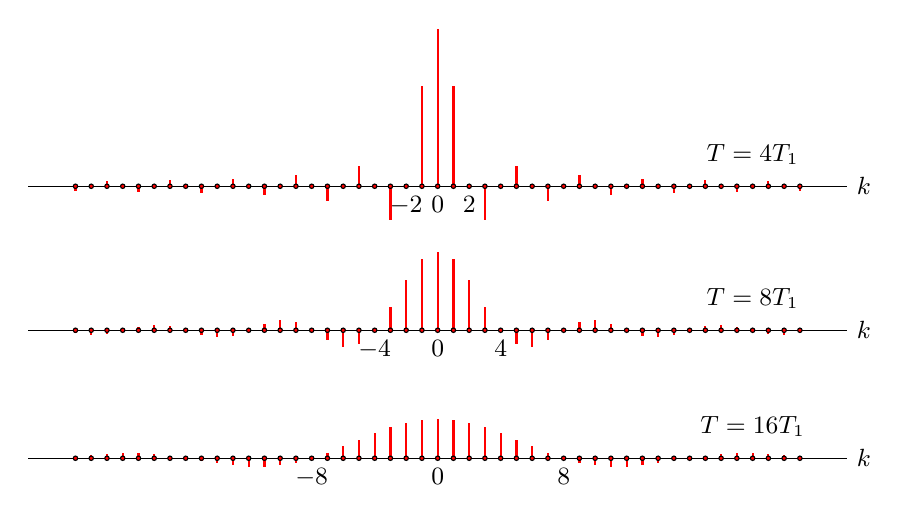
\begin{tikzpicture}[scale=0.4]
	\def\w{{-23,-22,-21,-20,-19,-18,-17,-16,-15,-14,-13,-12,-11,-10,-9,-8,-7,-6,-5,-4,-3,-2,-1,0,1,2,3,4,5,6,7,8,9,10,11,12,13,14,15,16,17,18,19,20,21,22,23}}
	\def\akmag{{-0.013840,0.000000,0.015158,-0.000000,-0.016753,0.000000,0.018724,-0.000000,-0.021221,0.000000,0.024485,-0.000000,-0.028937,0.000000,0.035368,-0.000000,-0.045473,0.000000,0.063662,-0.000000,-0.106103,0.000000,0.318310,0.500000,0.318310,0.000000,-0.106103,-0.000000,0.063662,0.000000,-0.045473,-0.000000,0.035368,0.000000,-0.028937,-0.000000,0.024485,0.000000,-0.021221,-0.000000,0.018724,0.000000,-0.016753,-0.000000,0.015158,0.000000,-0.013840}}


	\begin{scope}	
		\draw (-13, 0) -- (13,0) node[anchor=west] {\small $k$};
		\foreach \k in {-2, 0, 2}
		{
			\node at (\k/2, 0) [anchor=north] {\small $\k$};
		}
		%\node at (0,5) [anchor=south] {\small $Ta_k$};
		
		\foreach \k in {0,1, ..., 46}
		{
			\pgfmathparse{\w[\k]/2}
			\edef\wk{\pgfmathresult}
			\pgfmathparse{\akmag[\k]}
			\edef\akmagk{\pgfmathresult}	
			\draw[thick, red] (\wk, 0) -- ++(0,10*\akmagk);% node [anchor=south] {\small $\akmagk$};
			\ifthenelse{\lengthtest{0 pt = \akmagk pt}}{\draw[fill=red]  (\wk,0) circle (2pt);}{}
		}
			\node at (10, 1) {\small $T= 4T_1$};		
	\end{scope}


\def\akmag{{-0.009786,-0.014469,-0.010718,0.000000,0.011846,0.017684,0.013240,-0.000000,-0.015005,-0.022736,-0.017314,0.000000,0.020462,0.031831,0.025009,-0.000000,-0.032154,-0.053052,-0.045016,0.000000,0.075026,0.159155,0.225079,0.250000,0.225079,0.159155,0.075026,0.000000,-0.045016,-0.053052,-0.032154,-0.000000,0.025009,0.031831,0.020462,0.000000,-0.017314,-0.022736,-0.015005,-0.000000,0.013240,0.017684,0.011846,0.000000,-0.010718,-0.014469,-0.009786}}


	\begin{scope}[yshift=-1.8in]
		\draw (-13, 0) -- (13,0) node[anchor=west] {\small $k$};
		\foreach \k in {-4, 0, 4}
		{
			\node at (\k/2, 0) [anchor=north] {\small $\k$};
		}
		%\node at (0,5) [anchor=south] {\small $Ta_k$};
		
		\foreach \k in {0,1, ..., 46}
		{
			\pgfmathparse{\w[\k]/2}
			\edef\wk{\pgfmathresult}
			\pgfmathparse{\akmag[\k]}
			\edef\akmagk{\pgfmathresult}	
			\draw[thick, red] (\wk, 0) -- ++(0,10*\akmagk);% node [anchor=south] {\small $\akmagk$};
			\ifthenelse{\lengthtest{0 pt = \akmagk pt}}{\draw[fill=red]  (\wk,0) circle (2pt);}{}		
		}
			\node at (10, 1) {\small $T= 8T_1$};			
	\end{scope}

\def\akmag{{0.005296,0.010231,0.014004,0.015915,0.015478,0.012504,0.007165,-0.000000,-0.008121,-0.016077,-0.022622,-0.026526,-0.026735,-0.022508,-0.013535,0.000000,0.017402,0.037513,0.058816,0.079577,0.098027,0.112540,0.121812,0.125000,0.121812,0.112540,0.098027,0.079577,0.058816,0.037513,0.017402,0.000000,-0.013535,-0.022508,-0.026735,-0.026526,-0.022622,-0.016077,-0.008121,-0.000000,0.007165,0.012504,0.015478,0.015915,0.014004,0.010231,0.005296}}


	\begin{scope}[yshift=-3.4in]
		\draw (-13, 0) -- (13,0) node[anchor=west] {\small $k$};
		\foreach \k in {-8, 0, 8}
		{
			\node at (\k/2, 0) [anchor=north] {\small $\k$};
		}
		%\node at (0,5) [anchor=south] {\small $Ta_k$};
		
		\foreach \k in {0,1, ..., 46}
		{
			\pgfmathparse{\w[\k]/2}
			\edef\wk{\pgfmathresult}
			\pgfmathparse{\akmag[\k]}
			\edef\akmagk{\pgfmathresult}	
			\draw[thick, red] (\wk, 0) -- ++(0,10*\akmagk);% node [anchor=south] {\small $\akmagk$};
			\ifthenelse{\lengthtest{0 pt = \akmagk pt}}{\draw[fill=red]  (\wk,0) circle (2pt);}{}
		}
			\node at (10, 1) {\small $T= 16T_1$};			
	\end{scope}

% 	\begin{scope}[yshift=-1in]
% 		\draw (-4, 0) -- (4,0) node[anchor=west] {\small $k$};
% 		\foreach \k in {0,1, ..., 6}
% 		{			
% 			\pgfmathparse{\w[\k]}
% 			\edef\wk{\pgfmathresult}
% 			\pgfmathparse{\akarg[\k]}
% 			\edef\akargk{\pgfmathresult}	
% 			\pgfmathint{\wk}
% 			\edef\km3int{\pgfmathresult}
% 			\pgfmathsign{\akargk}
%             \def\argsign{\pgfmathresult}		
% 			\ifthenelse{-1=\argsign}{\node at (\wk, 0) [anchor=south] {\small $\km3int$};}{\node at (\wk, 0) [anchor=north] {\small $\km3int$};}
% 			\ifthenelse{-1=\argsign}{\edef\anchor{north}}{\edef\anchor{south}}			
%
% 			\draw[thick] (\wk, 0) -- ++(0,\akargk) node[anchor=\anchor] {\small $\akargk$};;
% 			\ifthenelse{\lengthtest{0 pt = \akargk pt}}{\draw[fill=black]  (\wk,0) circle (2pt);}{}			
% 		}
% 		%\node at (0,1.2) [anchor=south] {\small $\sphericalangle a_k$};				
% 	\end{scope}
\end{tikzpicture} 